%\documentclass[aspectratio=169]{beamer}
\documentclass{beamer}
\usepackage{graphicx,amsmath}
\usepackage{algorithmicx}
\usepackage{algorithm}
\usepackage{algpseudocode}
\usepackage{microtype}
\usepackage{tikz}
\usepackage{wrapfig}
\usepackage{bm}
\usepackage{soul}
\usepackage{subcaption}
\renewcommand{\vec}{\mathbf}
\usepackage{xcolor}
\renewcommand{\Re}{{\rm I\!R}}

\author[Maarten de Waard]{Maarten de Waard\\\small{Supervised by Diederik
	Roijers and Sander Bakkes}}
	\title[O-MCTS for GVGP]{Monte Carlo Tree Search with Options for General Video Game Playing}
\date{February 22\textsuperscript{nd}\\Public Thesis Defense}
\usetheme{Berkeley}

\begin{document}
\begin{frame}
	\vspace{-4.7em}
	\centerline{
	\includegraphics[scale=.8]{includes/LogoUvA}
	}
	%\hspace{1cm}
	%\vspace{-1cm}
	\maketitle
\end{frame}

\section{Introduction}

\begin{frame}
	\frametitle{Contents}
	\tableofcontents
\end{frame}

\begin{frame}
	\frametitle{Decision Theory \& General Video Game Playing}
	\begin{block}{Decision Theory}
		\begin{itemize}
			\item A general AI algorithm is capable of solving different problems
			\item Creating general AI algorithms is a step to \emph{strong AI}
		\end{itemize}
	\end{block}
	\begin{block}{General Video Game Playing}
		\begin{itemize}
			\item Games as problem setting
			\item Real world problems can be modelled as games
		\end{itemize}
	\end{block}
\end{frame}

\section{Background}

\subsection{Markov Decision Processes}
\begin{frame}
	\frametitle{Markov Decision Processes (MDPs)}
	States, actions, reward. Maximise cumulative reward over time.
	\begin{figure}
	\centering
	\includegraphics[height=.4\textwidth]{includes/mdp}
	\end{figure}
\end{frame}

\subsection{Monte Carlo Tree Search}
\begin{frame}
	\frametitle{Monte Carlo Tree Search}
	\begin{figure}
	\centering
	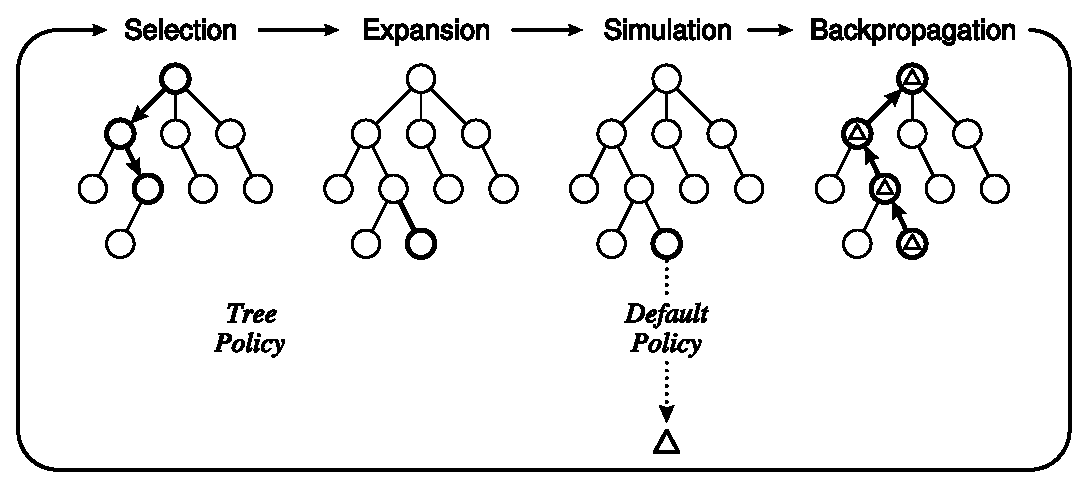
\includegraphics[height=.94\textheight]{includes/mcts}
	\end{figure}
\end{frame}

\subsection{Options}
\begin{frame}
	\frametitle{Options}
\end{frame}

\subsection{SMDP Q-learning}
\begin{frame}
	\frametitle{SMDP Q-learning}
\end{frame}

\subsection{General Video Game Playing}
\begin{frame}
	\frametitle{General Video Game Playing}
\end{frame}

\section{Options for GVGP}
\begin{frame}
	\frametitle{Game Description}
\end{frame}

\begin{frame}
	\frametitle{Option Set}
\end{frame}

\section{O-MCTS}
\begin{frame}
	\frametitle{Option MCTS}
\end{frame}

\section{OL-MCTS}
\begin{frame}
	\frametitle{Option Learning MCTS}
\end{frame}

\section{Experiments}
\begin{frame}
	\frametitle{SMDP Q-learning vs. MCTS}
	\begin{figure}
	\centering
	\makebox[\columnwidth]{\includegraphics[width=1.05\textwidth]{includes/qLearningWins}}
	\end{figure}
	\begin{figure}
	\centering
	\makebox[\columnwidth]{\includegraphics[width=1.05\textwidth]{includes/qLearningScores}}
	\end{figure}
\end{frame}

\begin{frame}
	\frametitle{O-MCTS vs. MCTS}
	\begin{figure}
	\centering
	\makebox[\columnwidth]{\includegraphics[width=1.05\textwidth]{includes/wins}}
	\end{figure}
	\begin{figure}
	\centering
	\makebox[\columnwidth]{\includegraphics[width=1.05\textwidth]{includes/scores}}
	\end{figure}
\end{frame}

\begin{frame}
	\frametitle{OL-MCTS vs. O-MCTS}
	\begin{figure}
	\centering
	\makebox[\columnwidth]{\includegraphics[width=1.05\textwidth]{includes/winsOLMCTS}}
	\end{figure}
	\begin{figure}
	\centering
	\makebox[\columnwidth]{\includegraphics[width=1.05\textwidth]{includes/scoresOLMCTS}}
	\end{figure}
\end{frame}

\begin{frame}
	\frametitle{Totals}
	\begin{figure}
	\centering
	\includegraphics[height=.6\textheight]{includes/totalsThesis}
	\end{figure}
\end{frame}

\section{Conclusion}
\begin{frame}
	\frametitle{O-MCTS}
\end{frame}

\begin{frame}
	\frametitle{OL-MCTS}
\end{frame}

\end{document}
